\subsection{Autoregressive Decoding and KV-Cache Memory Pressure}
Making large language models fast enough to deploy is still hard. Even with everything that has improved in text generation, summarization, and conversational assistants, this part of the problem has not really gone away. A big piece of it comes down to how expensive inference is, in compute and in memory. Size is not the only thing that decides model performance, how well execution stages and memory resources get managed during autoregressive attention matters just as much \cite{agrawal2023sarathi}.

LLM inference is commonly divided into two main phases: prefill and decode. In the prefill phase, all tokens in the input prompt get processed in parallel, to build the initial state required for generation. In the decode phase, output tokens get generated one by one, sequentially, so this stage is typically more constrained by memory bandwidth than by raw compute \cite{agrawal2023sarathi}.

Serving systems use something called the KV cache to avoid recomputing things across prefill and decode, storing the key and value vectors of the tokens already processed so the model does not have to redo that work every step. It helps a lot, but it is not free: as context length grows, or more requests run at once, or the expected output gets longer, the GPU memory pressure grows right along with it, and that pressure ends up shaping inference latency, batch size, and throughput all at once \cite{kwon2023pagedattention}. That is why we schedule around request size in memory blocks in this project, instead of raw token count. Every request object in our simulator carries its size in blocks, not tokens.

\subsection{PagedAttention and Block-Based Serving}
Allocating the KV cache in one contiguous block causes fragmentation, both internal and external, and that hurts memory utilization and caps how many requests fit at once. PagedAttention fixes this by breaking the KV cache into fixed-size blocks stored in non-contiguous memory \cite{kwon2023pagedattention}. The idea borrows from paging in operating systems. It works. Allocation gets more flexible, memory gets used better. LayerKV pushes the idea further, modeling the cache at the layer level instead of just the request level \cite{xiong2024layerkv}. Learned Prefix Caching looks at something else entirely: how prefix length and reuse patterns end up shaping memory allocation and eviction \cite{yang2024prefixcache}.

\begin{figure}[h]
  \centering
  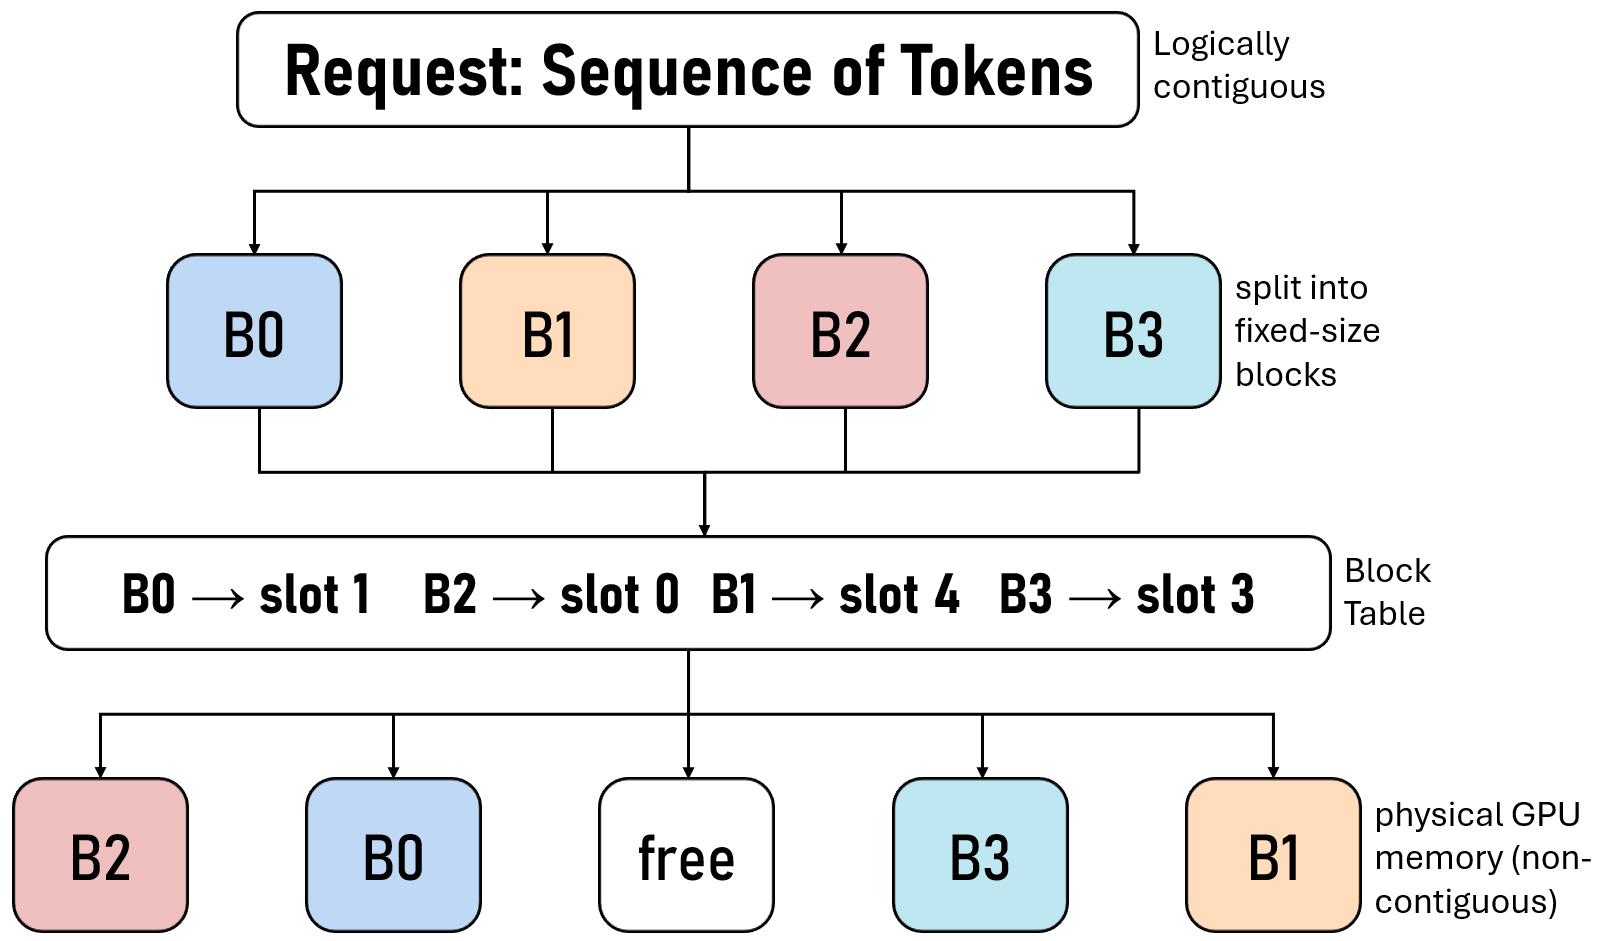
\includegraphics[width=\linewidth]{figures/fig_pagedattention.png}
  \caption{PagedAttention block mapping concept.}
  \label{fig:pagedattention}
\end{figure}

Our simulator uses the same block-based view of request size. The engine itself stays serial though, one request at a time, with no continuous batching, no real block pool, no eviction policy. That was a deliberate choice to keep the scope manageable, not something we missed, and we go back to it honestly as a limitation later, in the Discussion.

\begin{figure}[h]
  \centering
  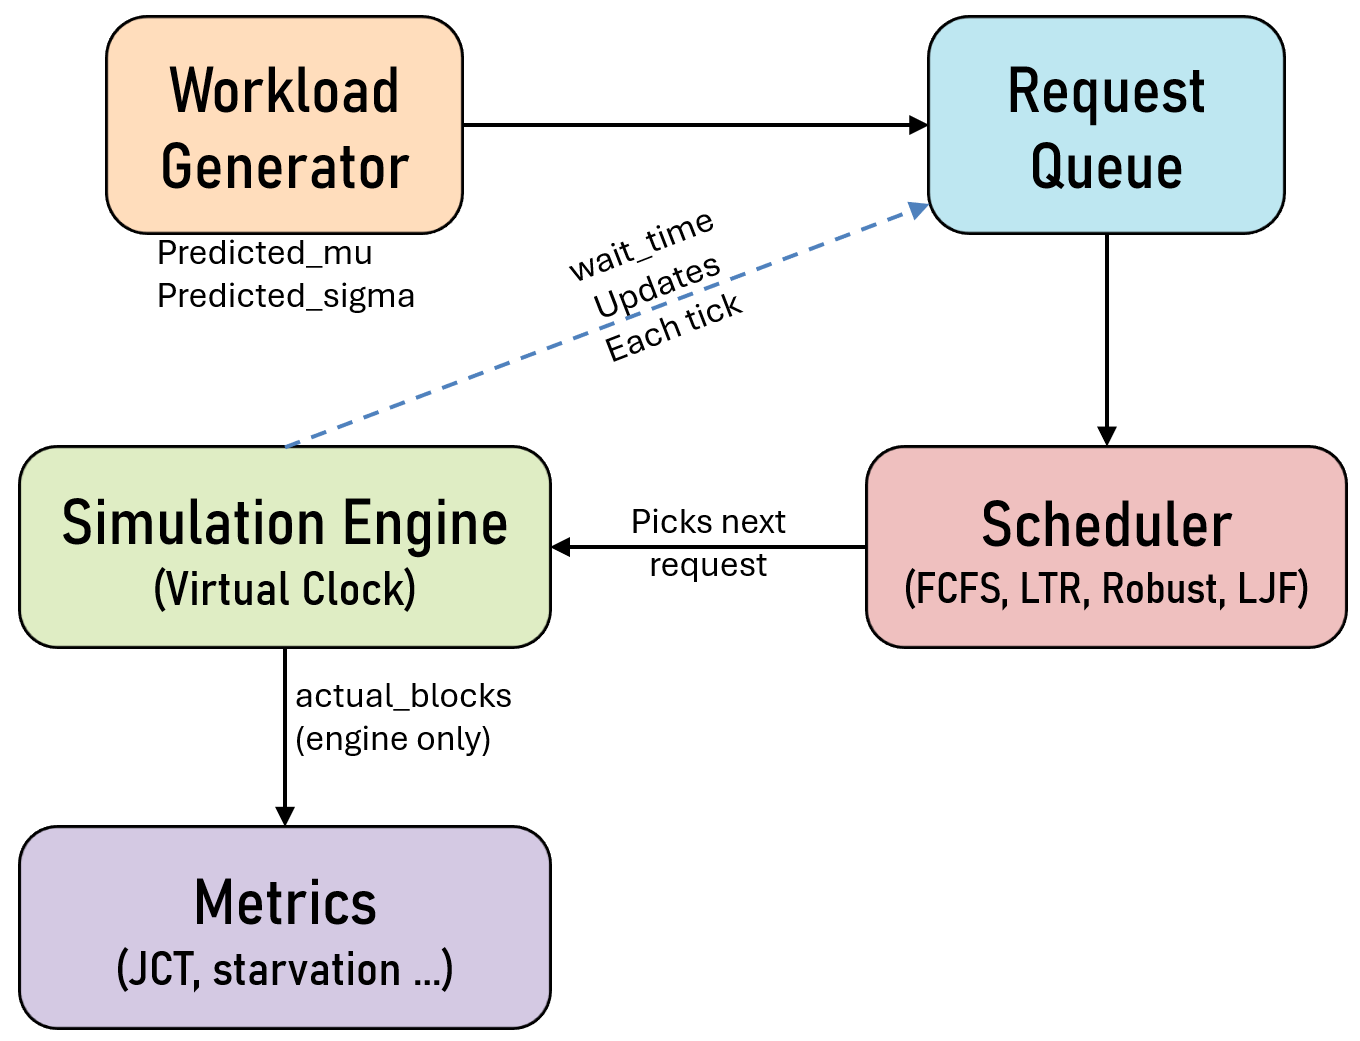
\includegraphics[width=\linewidth]{figures/fig_architecture.png}
  \caption{Simulator architecture pipeline.}
  \label{fig:architecture}
\end{figure}